\documentclass[10pt]{standalone}
\usepackage{amsmath}
\usepackage{amssymb}
\usepackage[utf8]{inputenc}
\usepackage{pgf,tikz,pgfplots}
\pgfplotsset{compat=1.15}
\usetikzlibrary{arrows}
\pagestyle{empty}
\begin{document}

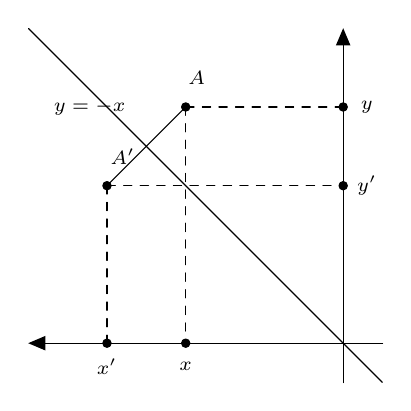
\begin{tikzpicture}[line cap=round,line join=round,>=triangle 45,x=1.0cm,y=1.0cm]
\draw[->] (0.5,0.) -- (-4.,0.);
;
\draw[->] (0.,-0.5) -- (0.,4.);
\clip(-4.,-0.5) rectangle (0.5,4.);
\draw [domain=-4.:0.5] plot(\x,{(-0.-1.*\x)/1.});
\draw (-3.,2.)-- (-2.,3.);
\draw [dash pattern=on 3pt off 3pt] (-2.,3.)-- (0.,3.);
\draw [dash pattern=on 3pt off 3pt] (-3.,2.)-- (0.,2.);
\draw [dash pattern=on 3pt off 3pt] (-2.,3.)-- (-2.,0.);
\draw [dash pattern=on 3pt off 3pt] (-3.,2.)-- (-3.,0.);
\begin{scriptsize}
\draw [fill=black] (0.,3.) circle (1.5pt);
\draw[color=black] (0.3,3.0) node {$y$};
\draw [fill=black] (0.,2.) circle (1.5pt);
\draw[color=black] (0.3,2.0) node {$y'$};

\draw [fill=black] (-2.,3.) circle (1.5pt);
\draw[color=black] (-1.86,3.37) node {$A$};
\draw [fill=black] (-3.,2.) circle (1.5pt);
\draw[color=black] (-2.8,2.37) node {$A'$};
\draw[color=black] (-3.22,3.0) node {$y=-x$};
\draw [fill=black] (-2.,0.) circle (1.5pt);
\draw[color=black] (-2.0,-0.3) node {$x$};
;
\draw [fill=black] (-3.,0.) circle (1.5pt);
\draw[color=black] (-3.0,-0.3) node {$x'$};
\end{scriptsize}

\end{tikzpicture}
\end{document}